\chapter{Experiments \label{cha:chapter4}}

\section{Dataset}


\subsection{MNIST}
MNIST\cite{LeCunMNISThandwrittendigit2010} is one of the most popular dataset that machine learning partitioners use to benchmark machine learning algorithms. The dataset consists of 60,000 training and 10,000 testing samples. Each sample is a grayscale 28x28 image of a digit between from 0 to 9. 

\begin{figure}[h]
\centering
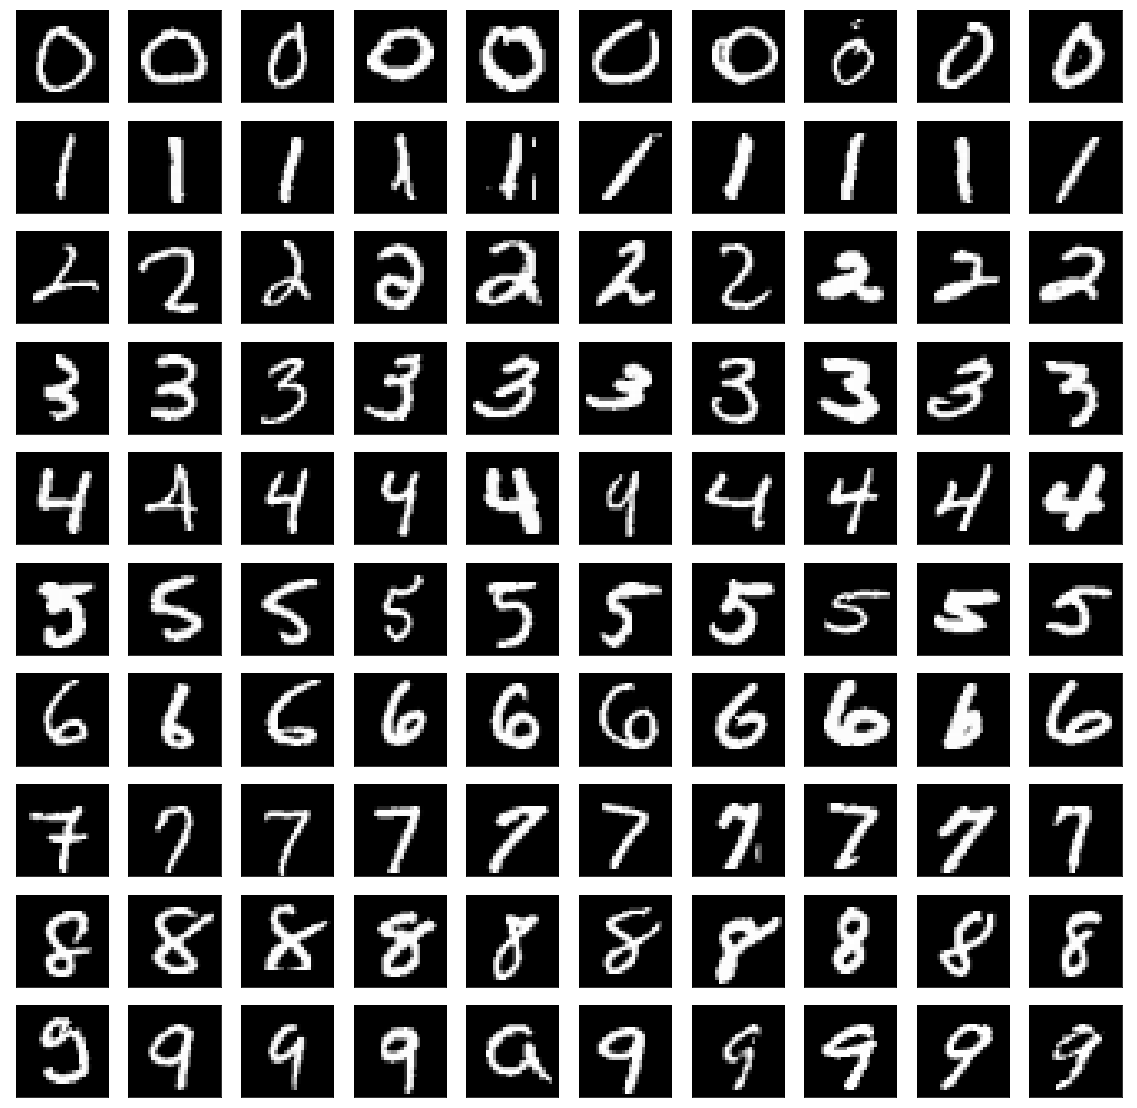
\includegraphics[width=0.5\textwidth]{mnist}
\caption{MNIST Dataset}
\label{fig:mnist_samples}
\end{figure}

State-of-the-art algorithms can classify MNIST with accuracy higher than 0.99, while classical ones, such as SVC or RandomForest, are able to achieve around 0.97\cite{XiaoFashionMNISTNovelImage2017}.


\subsection{Fashion-MNIST}

Xiao et. al.\cite{XiaoFashionMNISTNovelImage2017} propose a novel dataset, called Fashion-MNIST dataset, as a replacement of MNIST dataset for benchmarking machine learning algorithms.  According to \cite{XiaoFashionMNISTNovelImage2017},  Fashion-MNIST brings more challenging to the problem and more representative to modern computer vision tasks. It contains images of fashion products from 10 categories. Fashion-MNIST is comparable to MNIST in every aspects, such as the size of training and testing set, image dimension and data format, hence one can easily  apply existing algorithms that work with MNIST to Fashion-MNIST without any change.

\begin{figure}[h]
\centering
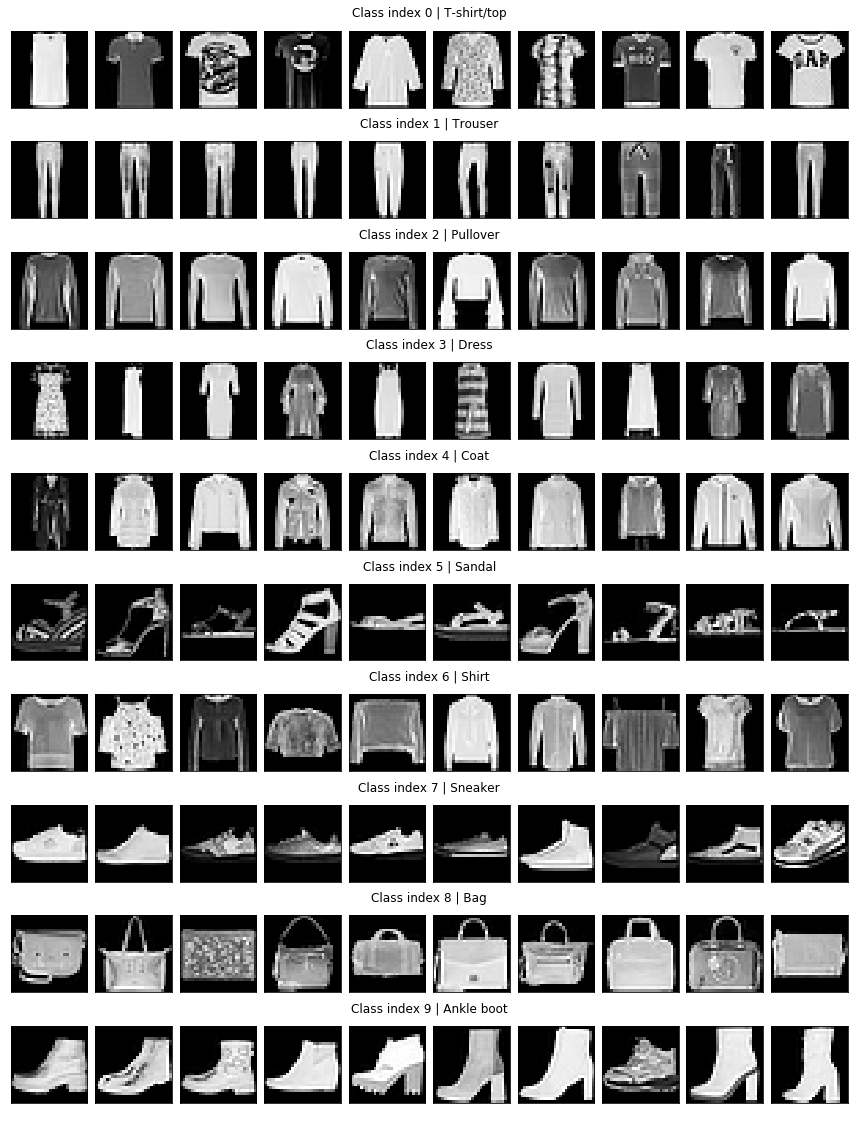
\includegraphics[width=0.6\textwidth]{fashion_mnist}
\caption{Fashion-MNIST Dataset}
\label{fig:mnist_samples}
\end{figure}

\cite{XiaoFashionMNISTNovelImage2017} also reports benchmarking results of classical machine learning algorithms on Fashion-MNIST. On average, they achieve accuracy between 0.85 to 0.89. According to Fashion-MNIST's page\footnote{https://github.com/zalandoresearch/fashion-mnist}, A. Brock reports the state-of-the-art result  with 0.97 accuracy using Wide Residual Network(WRN)\cite{ZagoruykoWideResidualNetworks2016} and standard data preprocessing and augmentation.

\section{The Problem}
 Because the main objective of the thesis is to demonstrate how well vanilla RNNs can propagate relevant quantity back to input space, we propose an artificial classification problem in which each sample is split into chunks and fed sequentially to the classifier. The classifier needs to summarize information along the sequence to make the final decision at the end. 
 
 \addfigure{\ref{fig:artificial_problem}} illustrates a general setting to the proposed problem. Here, a MNIST sample $ \patvector{x} \in \mathbb{R}^{28,28}$ is column-wise split into a sequence of $\{ \patvector{x}_t \}_{t=0} ^ 3, \patvector{x}_t \in   \mathbb{R}^{28,7}$. For a step $t$, $\patvector{x}_t$ is fed to a RNN cell, whose parameters denoted by $\patvector{\theta}$, yielding recurrent input $\patvector{r}_{t+1}$ for the next step. For the last step $t_{\text{last}} = 3$, we compute the final decision to the classification problem $\patvector{\hat{y}} \in \mathbb{R}^{10}$. 
 \begin{figure}[!hbt]
\centering
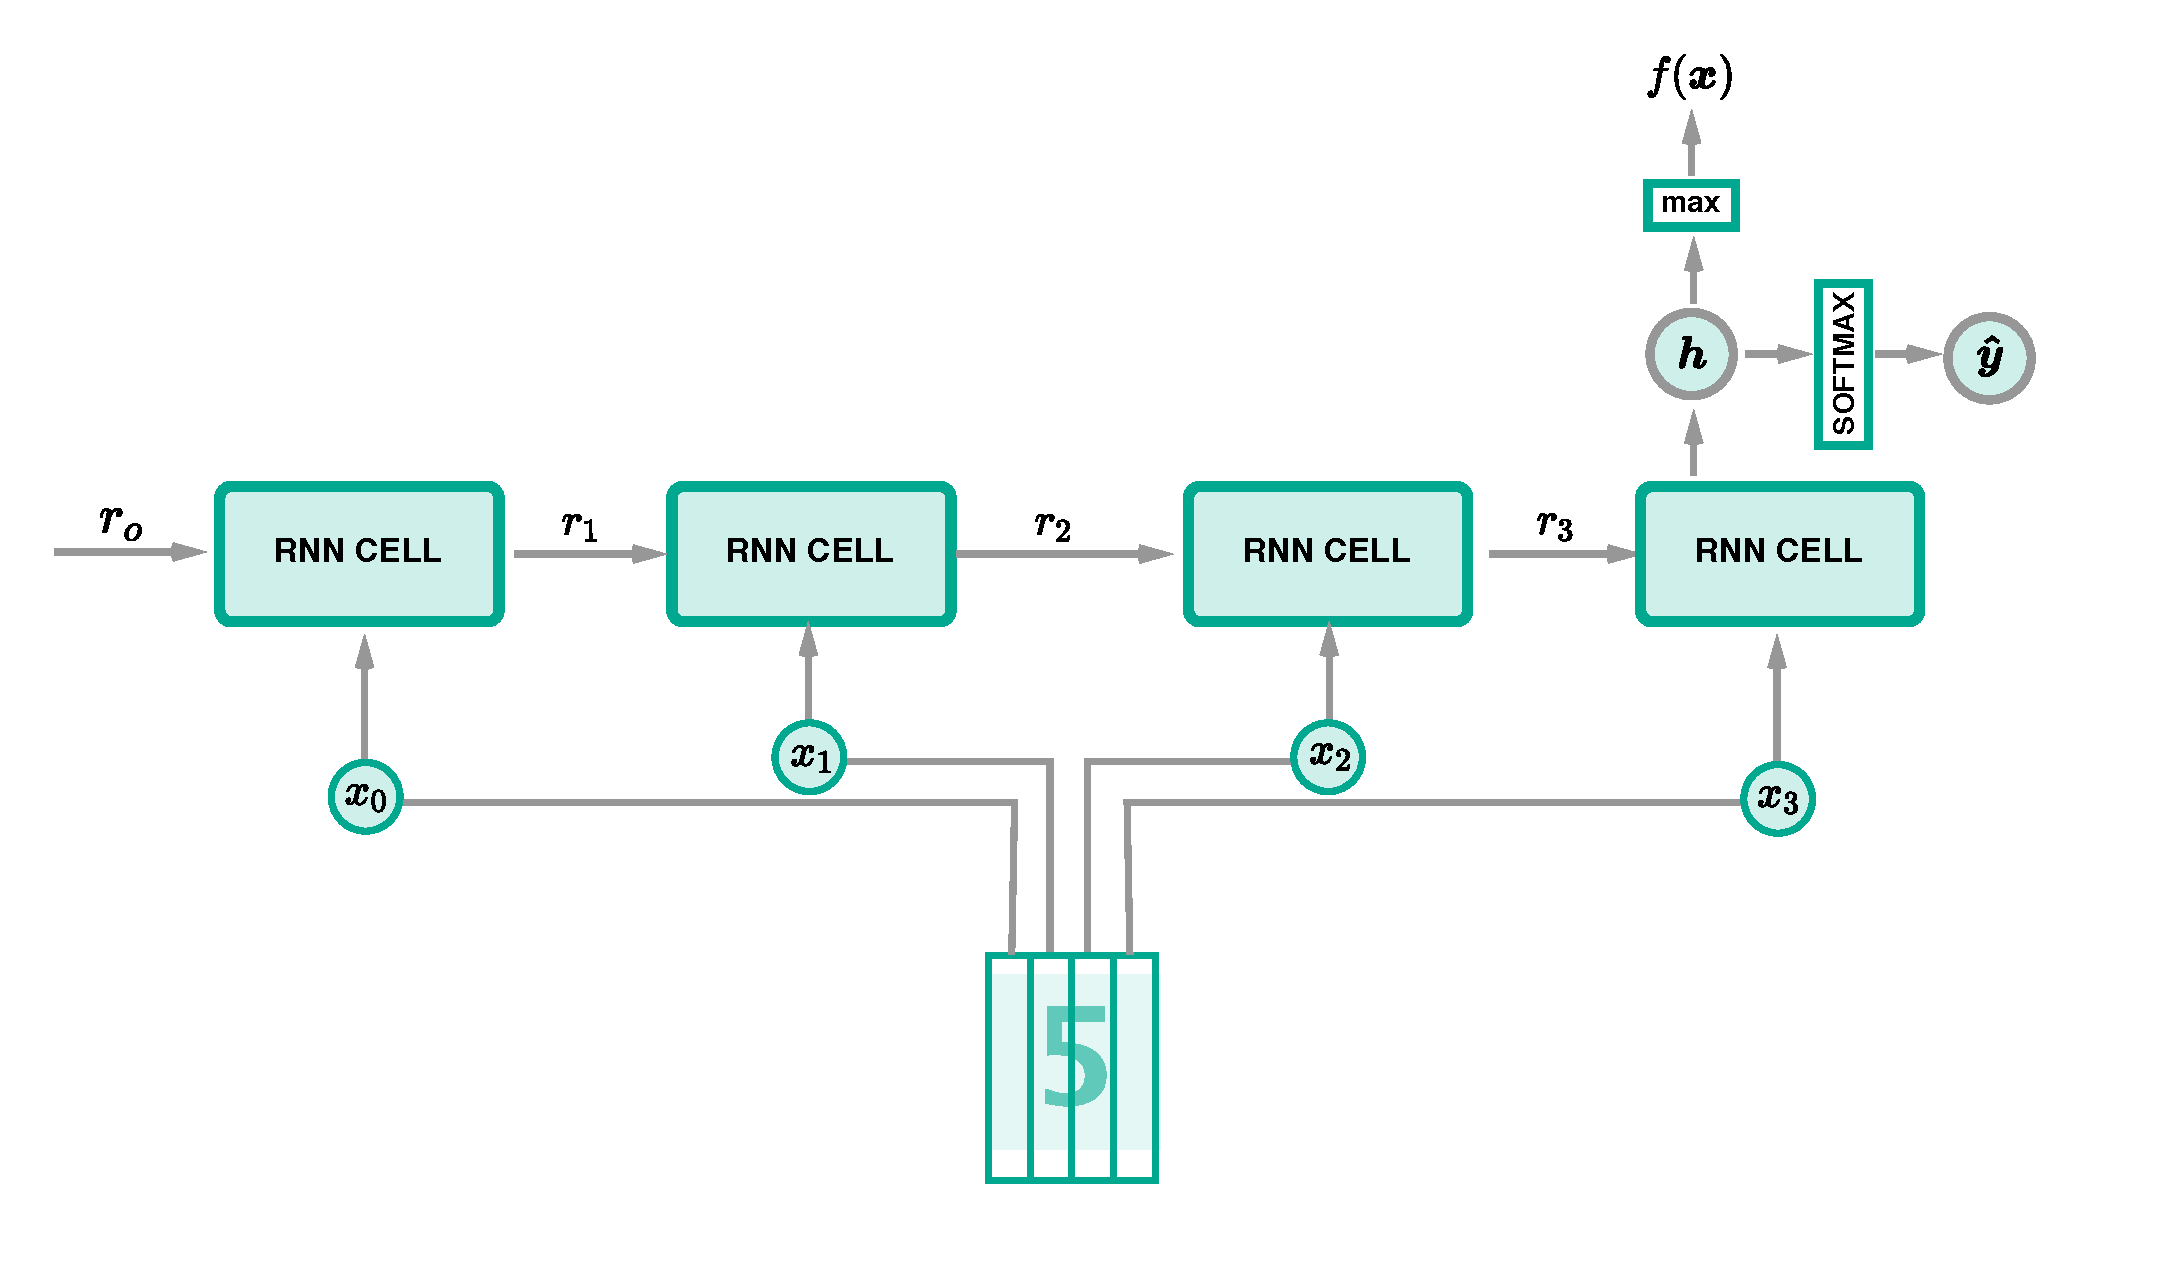
\includegraphics[width=0.9\textwidth]{sketch/artificial_problem}
\caption{General setting of RNN classifiers in this thesis} 
\label{fig:artificial_problem}
\end{figure}

 Denote $g_r$ and $g_{h}$ a function that a RNN cell uses to compute $\patvector{r}_{t+1}$ and raw output $\patvector{h} \in \mathbb{R}^{10}$ at the last step respectively. The whole computation can be summarized as follows: 
 \begin{align*}
 	\patvector{r}_{t+1} &= g_r(\patvector{\theta}, \patvector{x_t}, \patvector{r_t}) \\
 	 &\ \ \vdots\\
 	 \patvector{h} &= g_{h}(\patvector{\theta}, \patvector{x}_{t_{\text{last}}},  \patvector{r}_{t_{\text{last}}}) \\
 	\patvector{\hat{y}} &= \text{softmax}(\patvector{h}),
 \end{align*}
 where $\patvector{\hat{y}}$ is the class prediction probabilites and $\patvector{r}_0 = \patvector{0}$. In this case, the relevance score $f(\patvector{x})$ that will be propagated is:
 \begin{align*}
 	f(\patvector{x}) = \max_i h_i
 \end{align*}
 
 
 In this thesis, I performed experiments  using sequence length $ SEQ = \{1, 4, 7, 14\}$.
Table \ref{tab:seq-length} shows dimensions of $\patvector{x}_t$ for different sequence length.

\renewcommand{\arraystretch}{1.5}
\begin{table}[h]
\centering
\begin{tabular}{l|l|l|l|l|}
\cline{2-5}
                                            & \multicolumn{4}{c|}{Sequence Length}                                                               \\ \hline
\multicolumn{1}{|c|}{Dataset}               & \multicolumn{1}{c|}{1} & \multicolumn{1}{c|}{4} & \multicolumn{1}{c|}{7} & \multicolumn{1}{c|}{14} \\ \hline
\multicolumn{1}{|l|}{MNIST / Fashion-MNIST} &        $ \mathbb{R}^{28,28}  $              &          $ \mathbb{R}^{28,7}  $               &         $ \mathbb{R}^{28,4}  $               &          $ \mathbb{R}^{28,2}  $               \\ \hline
%\multicolumn{1}{|l|}{UFI-Cropped}           &                        &                        &                        &                         \\ \hline
%\multicolumn{1}{|l|}{}                      &                        &                        &                        &                         \\ \hline
\end{tabular}
\caption{Dimensions of $\patvector{x}_t$ for each dataset and sequence length}
\label{tab:seq-length}

\end{table}
\renewcommand{\arraystretch}{1}


\section{RNN Cell Architectures}
In this section, I will describe architectures or RNN cell evaluated in this thesis.  To make the descriptions concise, I denote notations as follows: 

\begin{itemize}
	\item $\patvector{a}_{t}^{(l)}$ : activation vector of layer $l$ at step $t$
	\item $\patvector{x}_t$ : subset of $x_i \in \patvector{x}$ corresponding to step $t$ and assume to be reshaped into a column vector
\end{itemize}

\subsection{Shallow Cell}
\begin{figure}[!htb]
\centering

\subfloat[Shallow cell\label{fig:s2_network}]{%
       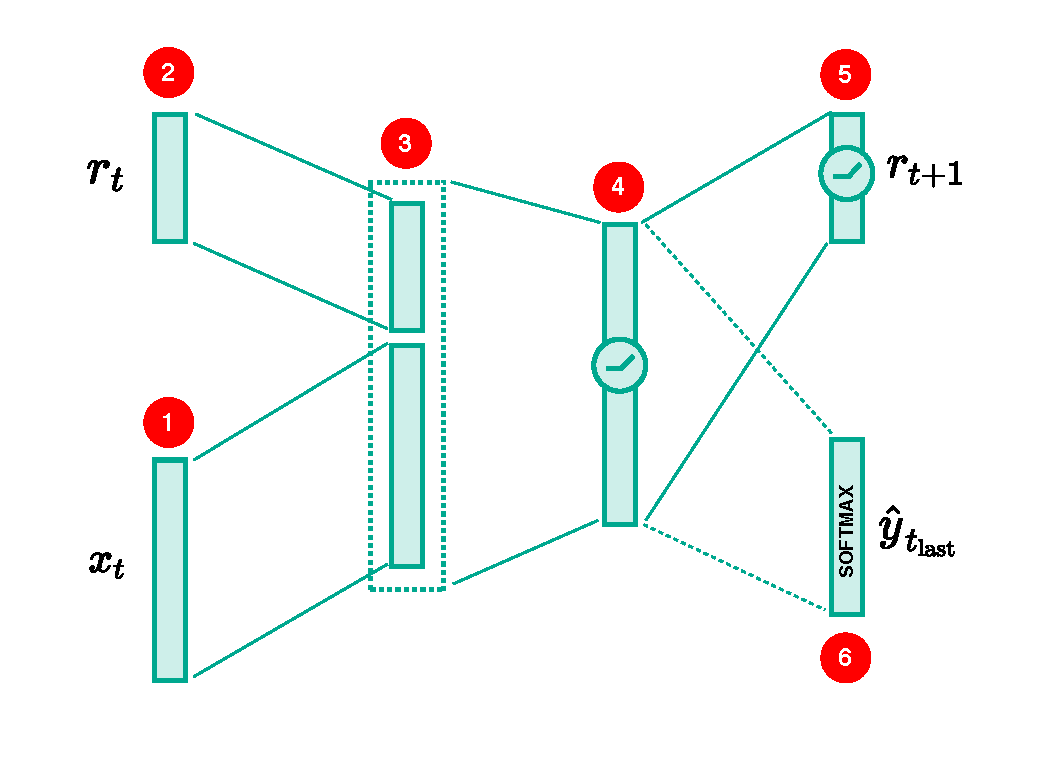
\includegraphics[width=0.48\textwidth]{sketch/s2_network}
     }
     \hfill
     \subfloat[Deep cell\label{fig:s3_network}]{%
       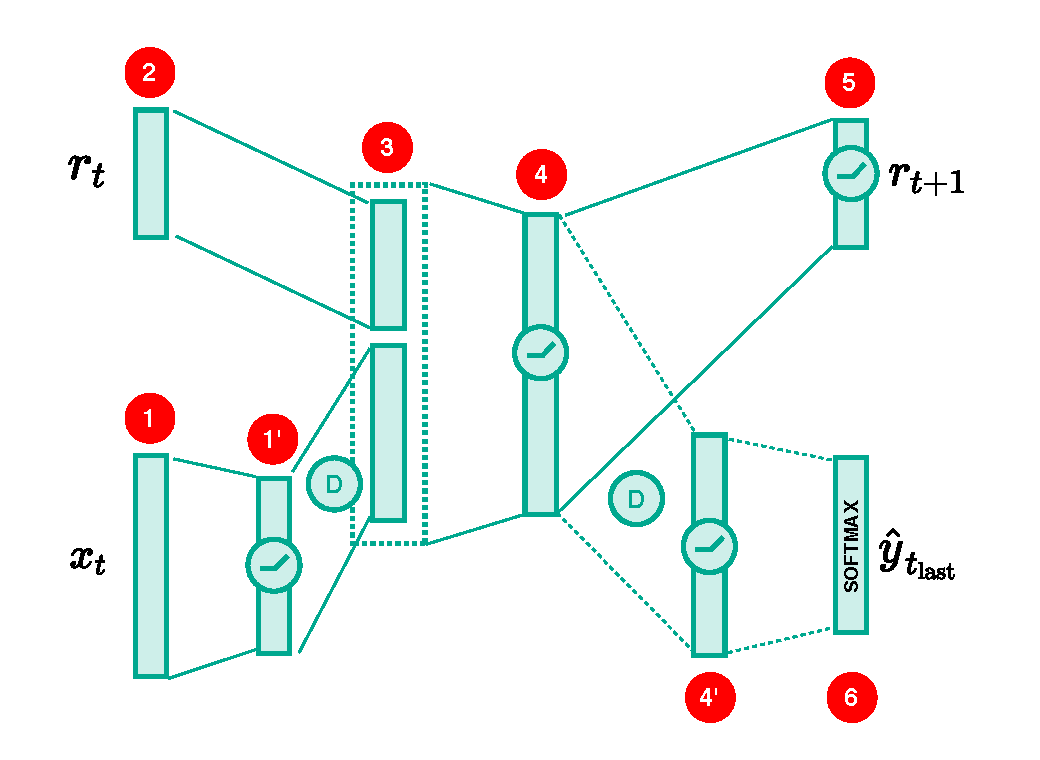
\includegraphics[width=0.48\textwidth]{sketch/s3_network}
     }
\caption{Shallow and Deep Cell Architecture}
\end{figure}

As shown in \addfigure{\ref{fig:s2_network}}, \rnncell{Shallow} cell first concatenates  input $\patvector{x}_t$  \circled{1} and recurrent input $\patvector{r}_t$  \circled{2} at layer \circled{3} as one vector before computing $\patvector{a}_t^{(4)} $ of layer \circled{4}. Then,  the next recurrent input $\patvector{r}_{t+1}$ \circled{5}	 is derived from $\patvector{a}_t^{(4)}$. In the last step $t_{\text{last}}$, the raw output $\patvector{h}$ is computed from $\patvector{a}^{(4)}_{t_{\text{last}}}$ and applied to softmax function to compute class probabilities $\patvector{\hat{y}}$ \circled{6}.



\subsection{Deep Cell Architecture}
%\begin{figure}[!htb]
%\centering
%
%\end{figure}

\addfigure{\ref{fig:s3_network}} illustrates the architecture of  \rnncell{Deep} cell. It can be viewed as  an extension of the Shallow cell with  2 additional layers, namely \circled{1'} and \circled{4'}.  The ideas of introducing the layers are to let \circled{1'} learn representations of the problem, while \circled{4} can focus on combining information from past and current step, which enables \circled{4'} to compute more fine-grained decision probabilities. Dropout is applied at $\patvector{a}^{(1')}_{\cdot}$, and $\patvector{a}^{(4)}_{t_\text{last}}$ for computing $\patvector{a}^{(4')}$.

\begin{figure}[!htb]
\centering

\subfloat[DeepV2\label{fig:deep_4l_network}]{%
       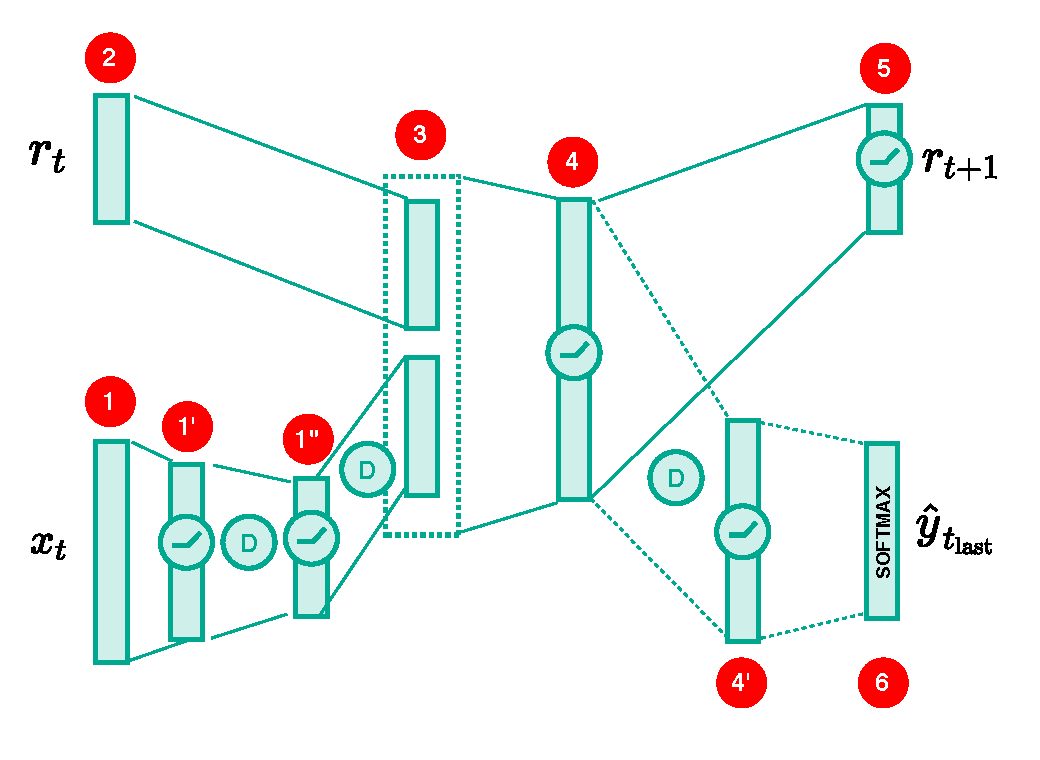
\includegraphics[width=0.48\textwidth]{sketch/deep_4l_network}
     }
     \hfill
     \subfloat[ConvDeep\label{fig:convdeep_4l_network}]{%
       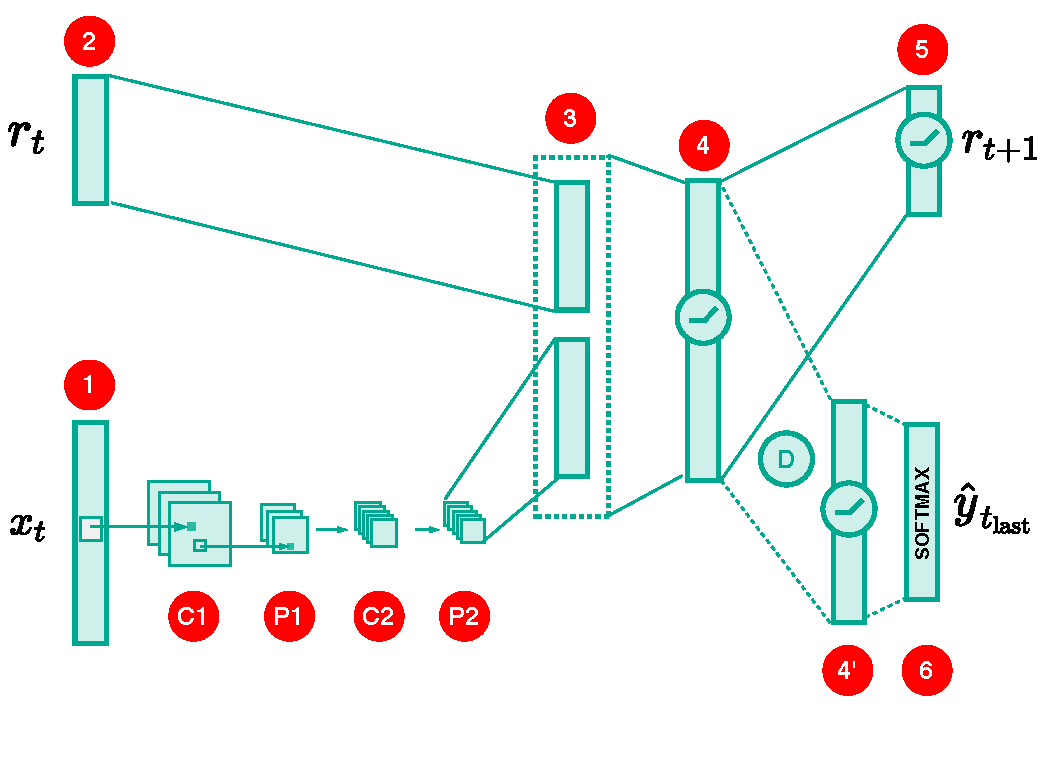
\includegraphics[width=0.48\textwidth]{sketch/convdeep_4l_network}
     }

\caption{DeepV2 and ConvDeep Cell Architecture}
\label{fig:deep_conv_arch}
\end{figure}
%
%
%
%\begin{figure}[!htb]
%\centering
%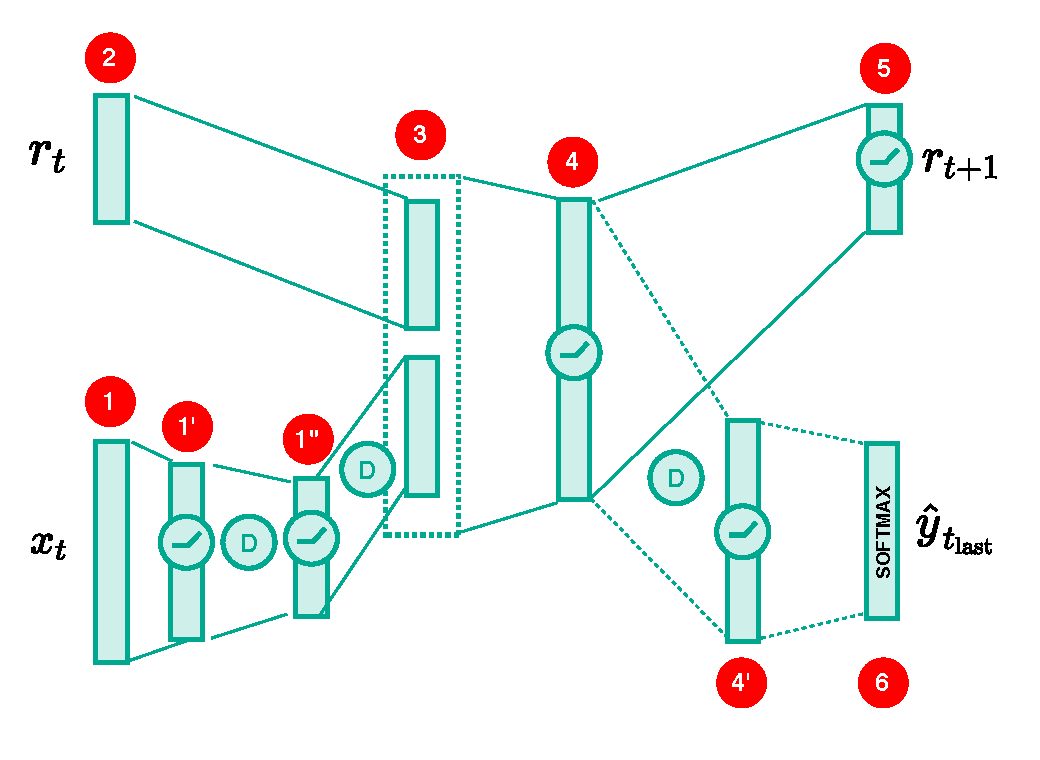
\includegraphics[width=0.6\textwidth]{sketch/deep_4l_network}
%\caption{DeepV2 Cell Architecture}
%\label{fig:deep_4l_network}
%\end{figure}
%
%
%\begin{figure}[!htb]
%\centering
%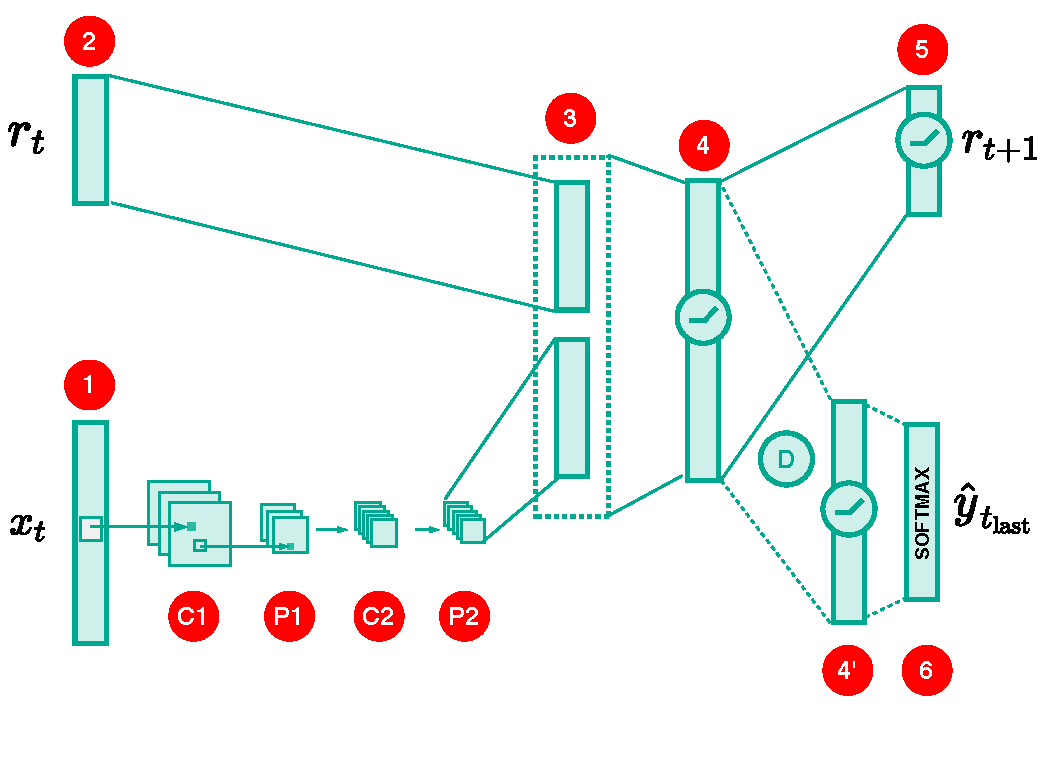
\includegraphics[width=0.6\textwidth]{sketch/convdeep_4l_network}
%\caption{ConvDeep Architecture}
%\label{fig:convdeep_4l_network}
%\end{figure}

Two variations of \rnncell{Deep} cell are also experimented, namely \rnncell{DeepV2} and \rnncell{ConvDeep}, shown on \addfigure{\ref{fig:deep_conv_arch}}. The former has one additional layer \circled{1"} with dropout regularization  between \circled{1'}. On the other hand, the latter replaces fully connected layers between \circled{1} and \circled{3} with 2 convolutional and max pooling layers, \Big[\circled{C1}, \circled{P1}\Big] and \Big[\circled{C2},\circled{P2}\Big].




\section{Setup}\label{sec:setup}
 
 I implemented experiments using TensorFlow\footnote{\url{http://tensorflow.org/}}.  weights $w_{ij} \in \patmatrix{W}$ and biases $b_{j} \in \patvector{b}$ are initialized as follows:
\begin{align*}
	w_{ij} &\sim \Psi( \mu=0, \sigma =0.1, [-2\sigma, 2\sigma]) \\
	b_{j} &= \ln(e^{0.01} - 1)
\end{align*}
where $\Psi(\cdot)$ denotes Truncated Normal Distribution with valid region between $[-2\sigma, 2\sigma]$.

%TODO : Figure normal distribution vs trucated

Activations $\patvector{a}^{(l)}_\cdot$ of layer $l$ is calculated using :
\begin{align*}
	\patvector{h}^{(l)}  &=  	\patmatrix{W}^T \patvector{a}^{(l-1)} - \sigma_{s}(\patvector{b}) \\
	\patvector{a}^{(l)}  &=  	\sigma_{r} (	\patvector{h}^{(l)} )
\end{align*}

where
\begin{align*}
	\sigma_{r} (h_j) &= \max(0, h_j)  \tag{ReLU function}\\
	\sigma_{s} (b_j) &= \log(1+\exp b_j) \tag{Softplus function}
\end{align*}
%TODO : Figure softplus vs relu

The reason of using $\sigma_{s} (b_j)$ for bias term is due to the non positive bias assumption of DTD. Moreover, $\sigma'_{s} (b_j)$ is $(0, \infty)$, as a result the network has more flexibility to adjust decision through back-propagation rather than using $\sigma_{r} (b_j)$. With this setting, the initial value of bias term  $\sigma_{s}(b_j)$ is then 0.01.

Speaking about training methodology, I use Adam\cite{KingmaAdamMethodStochastic2014} optimizer to train networks. Preliminary study shows that relevance heatmaps from networks trained by Adam are less noisy than the ones from other optimizers, such as  Stochastic Gradient Descent(SGD). Number of epochs is set to 200, while dropout probability is 0.5 and batch size is 50.  
Learning rate is not fixed as it is likely that different network architectures requires different value to achieve good performance, hence left adjustable. Table \ref{tab:hyper_summary} summaries the setting of hyperparameters.

%TODO: Heatmaps SGD, RMSProp, Adam
 
 \begin{table}[!htb]
\centering
\begin{tabular}{l|r}
\textbf{Hyperparameter} & \multicolumn{1}{l}{\textbf{Value}} \\ \hline
Optimizer               & Adam                               \\
Epoch     & 200                                \\
Dropout Probability     & 0.5                                \\
Batch size              & 50                                
\end{tabular}
\caption{Hyperparameter Summary}
\label{tab:hyper_summary}
\end{table}
 
Traditionally, number of neurons in each layer ($n^{(l)}$) is  another hyperparameter that we can adjust. However, as the goal is to compare relevance heatmaps from different architectures, those numbers are fixed and chosen in such a way that total number of variables in each architecture are equivalent. \addfigure{\ref{fig:neuron_numbers}} illustrates the details of the settings.

\begin{figure}[!htb]
\centering
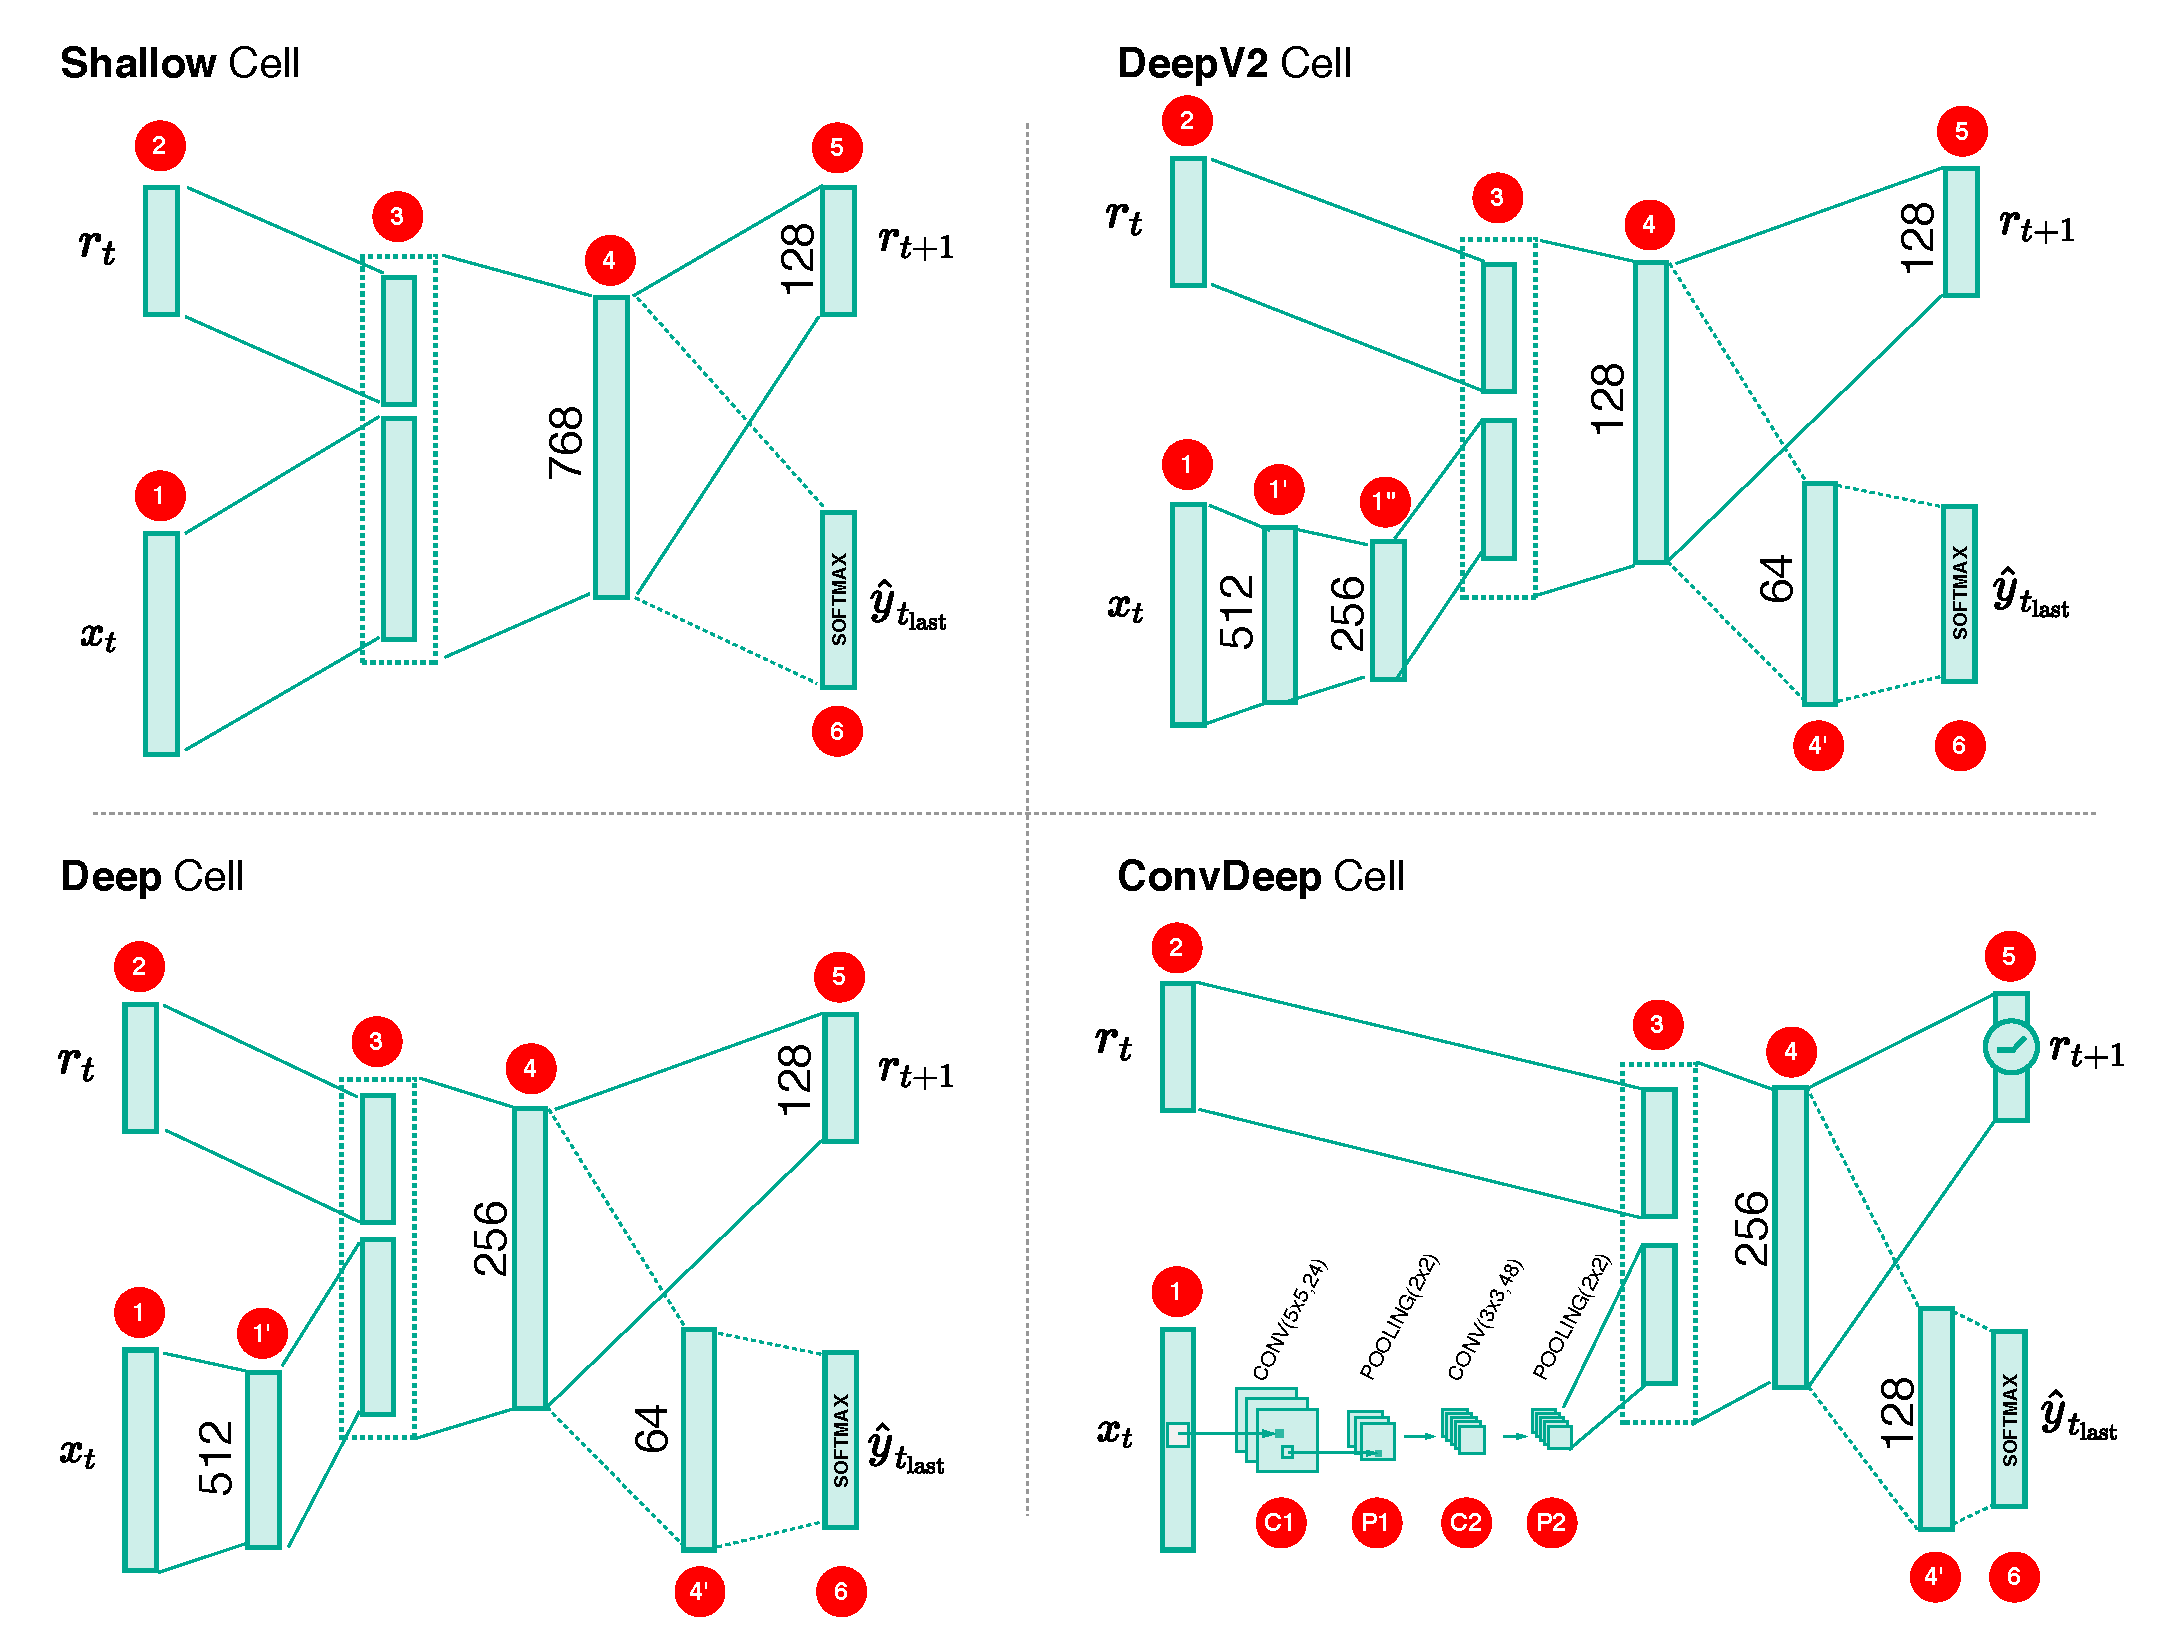
\includegraphics[width=\textwidth]{sketch/neuron_numbers}
\caption{Number of neurons in each layer for each cell architecture}
\label{fig:neuron_numbers}
\end{figure}


\begin{itemize}
	\item \textbf{Shallow Cell} 
$$\{ n^{(4)}\} = \{ 768 \}$$
	\item \textbf{Deep Cell} 
$$\{ n^{(1')}, n^{(4)}, n^{(4')} \} = \{ 512, 256, 64 \}$$
	\item \textbf{DeepV2 Cell} 
$$\{ n^{(1')}, n^{(1")}, n^{(4)}, n^{(4')} \} = \{ 512, 256, 128, 64 \}$$
	\item \textbf{ConvDeep Cell} : 
\begin{align*}
	\{ n^{(C1)}, n^{(P1)} \} &= \{ CONV(5\text{x}5, 24), POOL(2\text{x}2) \} \\
		\{ n^{(C2)}, n^{(P2)} \} &= \{ CONV(3\text{x}3, 48), POOL(2\text{x}2) \} \\
			\{  n^{(4)}, n^{(4')} \} &= \{ 256, 128 \}
\end{align*}
where $CONV(x,y)$ is a convolutional operator with $y$ filters whose kernel size is $\mathbb{R}^{x}$. Similarly, $POOL(x)$ is a pooling operator  with kernel size $\mathbb{R}^{x}$.


\end{itemize}

Noting that, $n^{(5)}$ is set at 128 for all architectures and 0 when the sequence length of the problem is 1. $n^{(6)}$ is equal to the number of categories of a problem, for example $n^{(6)} = 10 $ MNIST. Table \ref{tab:variable_architecture} shows the total numbers of variables in details.

\renewcommand{\arraystretch}{1.2}
\begin{table}[h]
\centering
\begin{tabular}{l|c|c|c|c|}
\cline{2-5}
                                                 & \multicolumn{4}{c|}{\textbf{Sequence Length}} \\ \hline
\multicolumn{1}{|l|}{\textbf{Cell Architecture}} & 1         & 4         & 7         & 14        \\ \hline
\multicolumn{1}{|l|}{\rnncell{Shallow}}                    & 610570    & 355722    & 291210    & 248202    \\ \hline
\multicolumn{1}{|l|}{\rnncell{Deep}}                       & 550346    & 314954    & 271946    & 243274    \\ \hline
\multicolumn{1}{|l|}{\rnncell{DeepV2}}                    & 575050    & 306890    & 263882    & 235210    \\ \hline
\multicolumn{1}{|l|}{\rnncell{ConvDeep}}                   & 647594    & 283178    & 197162    & 197162    \\ \hline
\end{tabular}
\caption{Total variables in each architecture and sequence length}
\label{tab:variable_architecture}
\end{table}


Lastly, as the quality of relevance heatmap depending on performance of the model, the minimum classification accuracy is set as in Table  \ref{tab:min_acc}. 

\begin{table}[h]
\centering
\begin{tabular}{ll}
\multicolumn{1}{l|}{\textbf{Dataset}} & \textbf{Minimum Accuracy} \\ \hline
\multicolumn{1}{l|}{MNIST}            & \multicolumn{1}{r}{0.98}  \\
\multicolumn{1}{l|}{Fashion-MNIST}    & \multicolumn{1}{r}{0.85}  \\
%\multicolumn{1}{l|}{UFI Cropped}                                       &                         \dots
\end{tabular}
\caption{Classification Accuracy Criteria}
\label{tab:min_acc}
\end{table}

% TODO : Hyper hopt Hyperopt

\section{Results}
In this section, I am going to present what I have  found from experiments. First, I am going to discuss results from MNIST and then move on to ones from Fashion-MNIST. Moreover, I will use \rnncellseq{CELL\_NAME}{SEQ} convention to denote a RNN network with CELL\_NAME cell trained on a sequence length SEQ. For example, \rnncellseq{Deep}{7} means a RNN with Deep cell architecture trained on data whose $\patvector{x}^{(\alpha)}$ is a sequence of length 7.
%TODO : More introduction

\subsection{MNIST}
As a starting point, I first trained classifiers using \rnncell{Shallow} and \rnncell{Deep} cell with $SEQ=\{1, 4, 7\}$ on MNSIT using setting described in Section \ref{sec:setup}. As shown in Table \ref{tab:mnist_model_acc}, these models are equivalent  in term of accuracy performance, hence their heatmaps can be compared. 

\begin{table}[]
\centering
\begin{tabular}{lrr}
\textbf{}                  & \multicolumn{1}{c}{\textbf{Shallow}} & \multicolumn{1}{c}{\textbf{Deep}} \\ \hline
\multicolumn{1}{l|}{SEQ-1} & 0.9813                               & 0.9788                            \\
\multicolumn{1}{l|}{SEQ-4} & 0.9830                               & 0.9861                            \\
\multicolumn{1}{l|}{SEQ-7} & 0.9807                               & 0.9852                           
\end{tabular}
\caption{Model Accuracy}
\label{tab:mnist_model_acc}
\end{table}

\addfigure{\ref{fig:mnist_experiment}} demonstrates relevance heatmaps from LRP and the trained models. Both \rnncellseq{Shallow}{1}  and \rnncellseq{Deep}{1} produce sound heatmaps, noting here that $\patvector{x}_t \in \mathbb{R}^{28,28}$. For $SEQ=\{4,7\}$,  their heatmaps are significantly different. \rnncellseq{Deep}{4,7}'s heatmaps contains high intensity values around the center of the images, while \rnncellseq{Shallow}{4,7}'s ones mostly concentrate on the right of the images.  This implies that \rnncellseq{Shallow}{4,7} are not able to  propagate relevance quantities through recurrent channels.

 \begin{figure}[h]
\centering
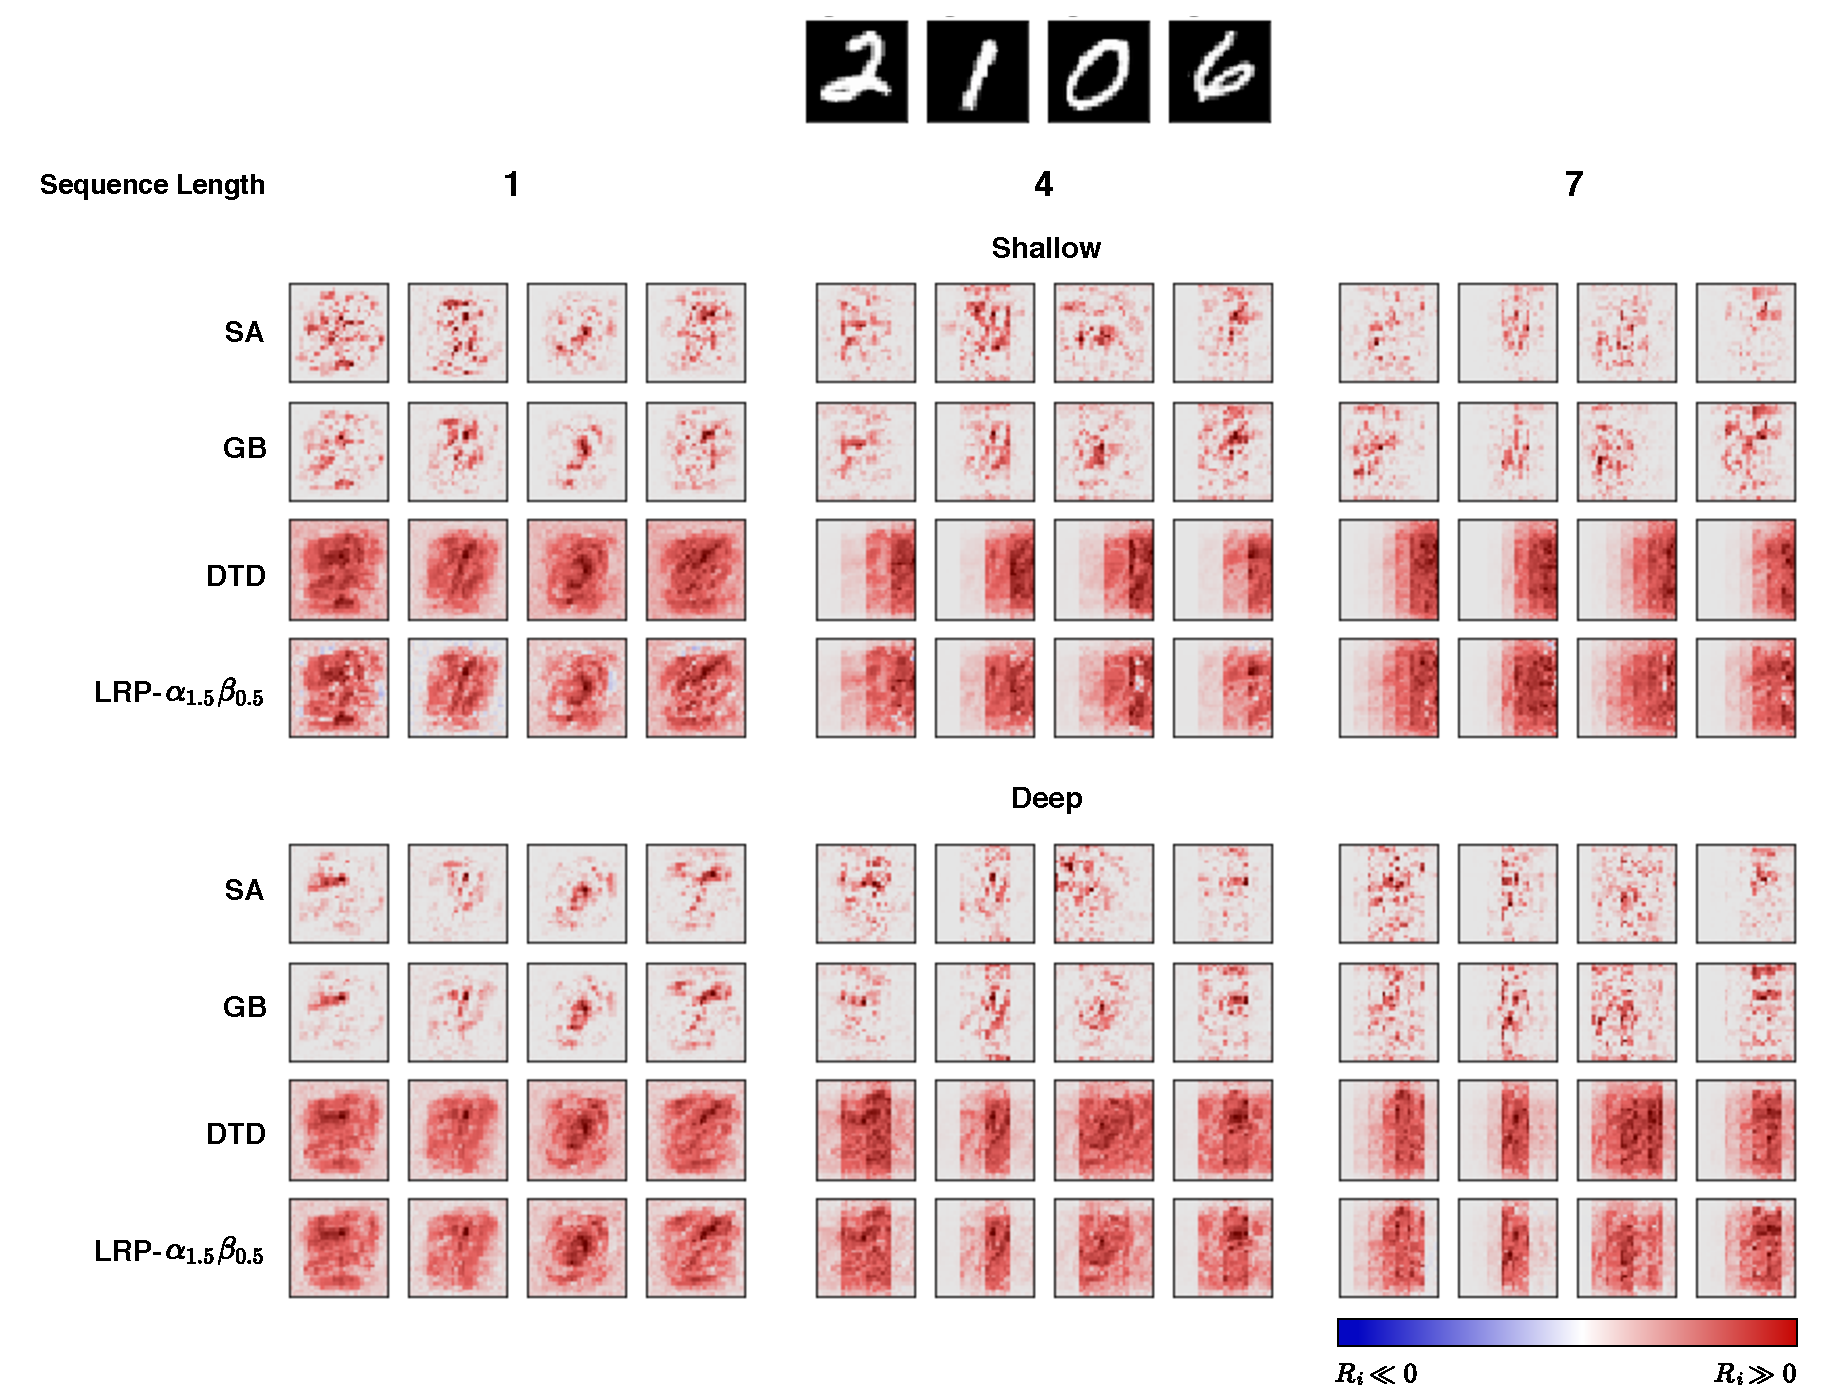
\includegraphics[width=\textwidth]{sketch/mnist_experiment}
\caption{Comparison of relevance heatmaps from LRP between Shallow and Deep Cell}
\label{fig:mnist_experiment}
\end{figure}

Moreover, we could observe that \rnncellseq{Deep}{4,7} are not only able to propagate relevance back through the input sequence, it also appropriately captures features of the input as the corresponding shapes of the samples are present on the heatmaps. On the other hand, \rnncellseq{Shallow}{4,7} do not show such capabilities.


 \begin{figure}[h]
\centering
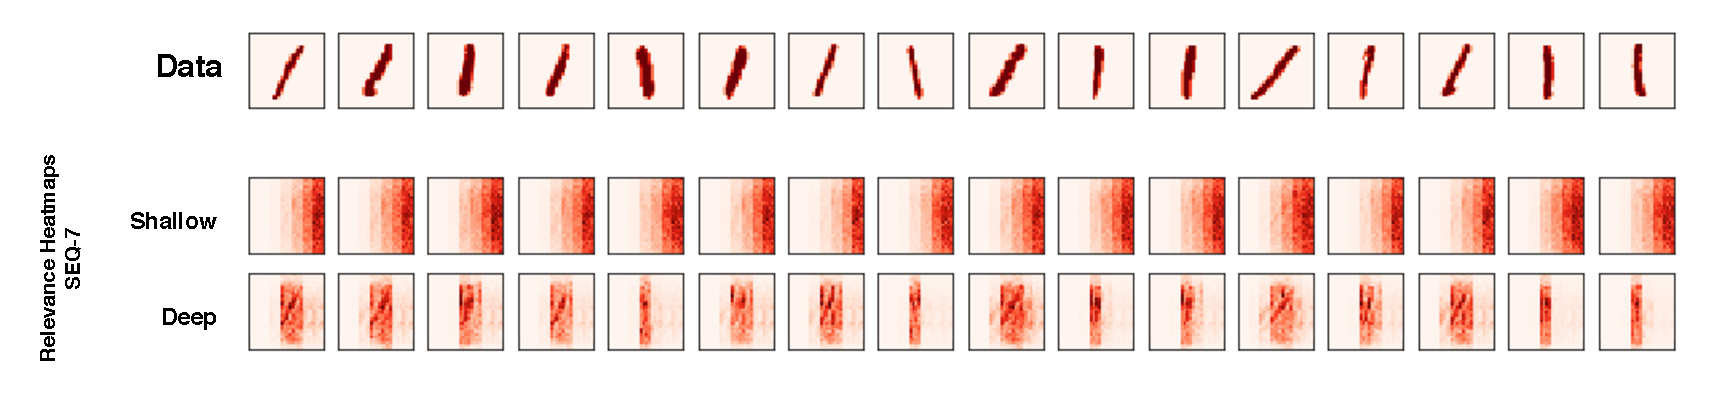
\includegraphics[width=\textwidth]{sketch/mnist_class_1_comparison}
\caption{Relevance heatmaps Shallow and Deep Cell\\(The samples are randomly chosen from MNIST's testing set)} 
\label{fig:mnist_experiment1}
\end{figure}

\addfigure{\ref{fig:mnist_experiment1}} shows more concrete evidence. Here, 16 samples from \textit{Class 1} were randomly chosen from the test set and fed to \rnncell{Shadow} and \rnncell{Deep} as  $SEQ=7$ meaning $\patvector{x}_t \in \mathbb{R}^{28,4}$.  Intuitively, the heatmaps from \rnncellseq{Deep}{7} align nicely to the data, while \rnncellseq{Shallow}{7}'s ones  do not seem to present any characteristic of the inputs. In fact, \rnncellseq{Deep}{7} manages to perfectly distribute relevance scores to region that the data actually lie, for example the last 2 images.  



\addfigure{\ref{fig:mnist_1_dist}}  also conveys the same insight, but from the aspect of  \textit{Class 1} population in testing set. The figure is a comparison of the distribution of pixel intensity from the \textit{Class 1} population, represented with dashed line, and the distributions of relevance quantities from the heatmaps explained by the models.  In the plot, value of the distribution for each step-$i^{th}$ is aggregated from corresponding pixels of the data and relevance heatmaps. We can clearly see that the distribution of relevance produced by \rnncellseq{Deep}{7}  looks similar to the input distribution, while the one from \rnncellseq{Shallow}{7} diverges significantly.


 \begin{figure}[h]
\centering
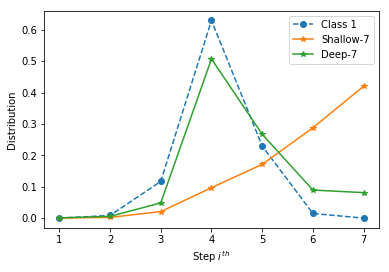
\includegraphics[width=0.5\textwidth]{notebooks/mnist_1_dist}
\caption{Comparison of pixel intensity distribution from MNIST Class 1 testing population and relevance distribution explained by the models} 
\label{fig:mnist_1_dist}
\end{figure}

It is worth mentioning that samples in MNIST Class 1 are relatively simples, hence comparing such distributions can give some insight of the explainability of the models. However, in real world setting, qualifying explainability of a neural network via the distributions might not give meaningful intuition, because input tends to have complex structure and the network is likely to produce relevance heatmap that has different structure from the original image. We shall see this behavior in Fashion-MNIST experiments.

% TODO : mention AOPC?




However, one intesting observation I have found is that senstitvity analysis ... 
\subsection{Fashion-MNIST}


%TODO : Add Model accuracy in appendix
